% !TeX document-id = {58d4c0c1-a5c3-4ae8-8c87-8b1ea6ea06a9}
\documentclass[a4paper,12pt,oneside]{book}
%-----------------------------------------------
%package
%-----------------------------------------------
\usepackage[english]{babel}
\usepackage[utf8]{inputenc}
\usepackage{amsmath}
\usepackage{textcomp}
\usepackage{amsfonts}
\usepackage{amssymb}
\usepackage[T1]{fontenc}
\usepackage{graphicx}
\usepackage{float}
\usepackage{siunitx}
\usepackage{subfigure}
\graphicspath{{foto/}}
\usepackage{colortbl}
\usepackage{color}
\usepackage{xcolor}
\usepackage{verbatim}
\usepackage{footmisc}
\usepackage[citecolor=black, filecolor=blue, linkcolor=blue, urlcolor=blue, colorlinks=true] {hyperref}
\usepackage{multirow}
\usepackage[font=small, format=hang, labelfont={bf}]{caption}
\usepackage{multicol}
\usepackage{listings}
\usepackage{makecell}
\usepackage{enumitem}	
\usepackage{titletoc}
\usepackage{minted}

% !TeX TXS-program:compile = txs:///lualatex/[--shell-escape]
\usemintedstyle{manni}
\definecolor{bgcode}{rgb}{0.97,0.97,0.97}

\interfootnotelinepenalty =10000
%-----------------------------------------------
%new command, colors, code listings
%-----------------------------------------------
%commands
\newcommand\tab[1][1cm]{\hspace{#1}}
\newcommand\C{^\circ C}
\newcommand\MatLab{\textsc{MatLab}}
\newcommand\smsr{\textsc{Smsr}}
\newcommand\fwhm{\textsc{Fwhm}}
\newcommand\osa{\textsc{Osa}}
\newcommand\esa{\textsc{Esa}}

%fancy
\usepackage{fancyhdr}
\pagestyle{fancy}
\chead{}
\cfoot{\thepage}
\lhead{}
\renewcommand{\headrulewidth}{0.4pt}
\renewcommand{\footrulewidth}{0.4pt}
\makeatletter 

\renewcommand{\@makechapterhead}[1]{% 
\vspace*{30 pt}% 
{\setlength{\parindent}{0pt} \raggedright \normalfont 
\bfseries\Huge 
\ifnum \value{secnumdepth}>1 
   \if@mainmatter\thechapter.\ \fi% 
\fi 
#1\par\nobreak\vspace{40 pt}}} 
\makeatother
\renewcommand{\chaptermark}[1]{%
\markboth{#1}{}}
\makeatletter 

%definizione figure
\usepackage[labelfont={bf}, font={small}, justification={centerlast}]{caption}

\usepackage{listings}
\usepackage{color} %red, green, blue, yellow, cyan, magenta, black, white
\definecolor{mygreen}{RGB}{28,172,0} % color values Red, Green, Blue
\definecolor{mylilas}{RGB}{170,55,241}
\lstset{language=Matlab,%
    breaklines=true,%
    morekeywords={void},
    keywordstyle=\color{blue},%
    morekeywords=[2]{1}, keywordstyle=[2]{\color{black}},
    identifierstyle=\color{black},%
    stringstyle=\color{mylilas},
    commentstyle=\color{mygreen},%
    showstringspaces=false,%without this there will be a symbol in the places where there is a space
    numbers=left,%
    numberstyle={\tiny \color{black}},% size of the numbers
    numbersep=9pt, % this defines how far the numbers are from the text
    emph=[1]{for,end,break},emphstyle=[1]\color{black}, %some words to emphasise
    %emph=[2]{word1,word2}, emphstyle=[2]{style},    
}

%formato numeri titoli
\usepackage{titlesec, blindtext, color}
\definecolor{gray75}{gray}{0.75}
\newcommand{\hsp}{\hspace{10pt}}
\newfont{\chapterNumber}{eurb10 scaled 7000}

\titleformat{\chapter}[display]%
{\relax}{\mbox{}\marginpar{\vspace*{-\baselineskip}\color{gray75}\chapterNumber\thechapter}}{0pt}%
  {\huge\bfseries}[\normalsize\vspace*{.8\baselineskip}\titlerule]% 
  
\titleformat{\section}[hang]{\normalfont\bfseries}{\thesection\hsp\textcolor{gray75}{|}\hsp}{0pt}{\normalfont\bfseries\LARGE}

\titleformat{\subsection}[hang]{\normalfont\bfseries}{\thesubsection\hsp\textcolor{gray75}{|}\hsp}{0pt}{\Large\bfseries}

\titleformat{\subsubsection}[hang]{\normalfont\bfseries}{\thesubsubsection\hsp\textcolor{gray75}{|}\hsp}{0pt}{\large\bfseries}

\titleformat{\paragraph}[runin]{\normalfont\bfseries}{\theparagraph\hsp\textcolor{gray75}{|}\hsp}{0pt}{\normalfont\bfseries}

\titlespacing{\section}{0pt}{20pt}{6pt}
\titlespacing{\subsection}{0pt}{15pt}{2pt}
\titlespacing{\subsubsection}{0pt}{15pt}{2pt}
\titlespacing{\paragraph}{0pt}{15pt}{10pt}

\setcounter{secnumdepth}{6}
\setcounter{tocdepth}{6}

%definizione parametri pagina 
\usepackage{geometry}
\geometry{a4paper,top=4cm,bottom=3.5cm,left=2.5cm,right=2.5cm}

%colors
\definecolor{mygray}{rgb}{0.5,0.5,0.5}

%highlight code
\lstdefinestyle{C}{
	language		= C,
	basicstyle		= \ttfamily,
	keywordstyle	= \color{blue}\ttfamily,
	stringstyle		= \color{red}\ttfamily,
	commentstyle	= \color{green}\ttfamily,
	morekeywords	= {for, },
	morecomment		= [l][\color{magenta}]{\#},
}
\lstdefinestyle{VHDL}{
	language     = VHDL,
	basicstyle   = \ttfamily,
	keywordstyle = \color{blue!100!black!80}\bfseries,
	commentstyle = \color{green!90!black!90},
	morekeywords={ library,use,all,entity,is,port,in,out,end,architecture,of,
	begin,and},
	morecomment=[l]--
}

%to force a line break in a table (package makecell)
\renewcommand\theadalign{bc}
\renewcommand\theadfont{\bfseries}
\renewcommand\theadgape{\Gape[4pt]}
\renewcommand\cellgape{\Gape[4pt]}

%-----------------------------------------------
%Title and first informations:
%-----------------------------------------------




%-----------------------------------------------
%document
%-----------------------------------------------
\begin{document}
%-----------------------------------------------
%Title and index in the document
%-----------------------------------------------

\tableofcontents
\listoffigures

%This way the first page is the title page, the second the index page and from the next page starts the real document
\newpage


%-----------------------------------------------
%Instruments
%-----------------------------------------------


%-----------------------------------------------
%chapters
%-----------------------------------------------

\mainmatter

\chapter{Introduction}
\graphicspath{{foto/Chap1/}}
\section{Introduction to the laboratory experience}
This project aims to estimate the characteristics of a 3D NAND memory array based on Traditional Planar Transistors through a MATLAB script.

The outputs of the model are:
\begin{itemize}[noitemsep, topsep=0pt]
\item Delay during a precharge and read operation
\item Power consumption due to a read operation
\item Power consumption due to a write operation
\item Power consumption due to an erase operation
\item Area and Volume
\end{itemize}

\section{Structure explanation}
The 3D NAND memory exploits the vertical dimension to increase the bit density of the array. From a logical point of view, the model is represented by a series of memory blocks called "slices" that together form the array, as shown in fig. \ref{fig:memory}. Every slice works like a traditional planar NAND memory block. So, after selecting a slice, the behaviour of the memory is the same as a planar one. All around the memory slices there are some pieces of circuit (Decoders) used to select the desired memory cell, plus other circuits, like Sense Amplifiers and Precharge Units, as shown in fig. \ref{fig:3dmemory}.

\begin{figure}[H] 
	\begin{center}
		\includegraphics[width=0.85\textwidth]{memory}
	\end{center}
	\caption{Block structure of the memory} 
	\label{fig:memory}
\end{figure} 

The elements that dissipate energy are:

\begin{itemize}
\item String select line (SSL)
\item Ground select line (GSL)
\item Bitlines (BLs)
\item Wordlines (WLs)
\item Slice enable transistors (SETs)
\item String select transistor (SST)
\item Ground select transistor (GST)
\item Floating gate transistors (FGTs)
\end{itemize}

\begin{center}
	\begin{figure}[H]
		\centering
		\includegraphics[scale = 0.55]{3dmemory-GENERAL_SCHEMATIC}
		\caption{Block diagram of the total structure}
		\label{fig:3dmemory}
	\end{figure}
\end{center}

\section{Behavior of the memory}
The behaviour of the memory can be modelled like a FSM with these states, as shown in fig. \ref{fig:fsm}:

\begin{itemize}[noitemsep, topsep=0pt]
\item Precharge
\item Read
\item Write
\item Erase
\end{itemize}

\begin{center}
	\begin{figure}[H]
		\centering
		\includegraphics[scale = 0.6]{FSM}
		\caption{State machine for memory operation}
		\label{fig:fsm}
	\end{figure}
\end{center}

\textbf{Precharge} is the initial state to perform a \textbf{read}, \textbf{write} or \textbf{erase} operation. During the precharge state, bitlines are biased at a certain voltage to speed up subsequent operations. Bitlines are electrically disconnected from the memory array because the SSL signal is not asserted. Thanks to slice enable transistors (SETs), the wordlines are electrically disconnected too.

\textbf{Read} and \textbf{Write} operations are performed at page level while erase at slice level. During any operation, unselected slices are electrically disconnected by the slice decoder.\\

The memory array in standard planar NAND is obviously a plane but in 3D ones it has a cubic shape. The cube is organized in blocks that in the model are referred to as \textit{slices}. A slice decoder is used to select only the desired slice and to electrically isolate the others.

The layout is organized in rows (\textit{wordlines}) and columns (\textit{bitlines}). At the intersection of each row and column there is a Floating Gate Transistor (FGT) that is the actual memory element. In the project a SLC (single-level cell) flash is used so each FGT stores only one bit of data. The FGTs connected in series form a \textit{string} and can be accessed using the String Select Transistor (SST) and the Ground Select Transistor (GST). The group of FGTs along the same WL is called \textit{page} and it is selected using the page decoder.

Flash memory exploits Tunneling Effect to perform write/erase operations on the FGTs. The write operation moves the tunneling charges in the floating gate, while they are extracted from it during the erase phase.\\

The model of the memory incudes also all the peripheral components needed to select the bits and to read them: apart from the memory slices, so, we have modelled also the slice, the row and column decoders, the sense amplifiers and all the pass transistors needed for the correct selection of the lines and for providing the data towards the external world. The behaviour of each component during a read operation will be better detailed in chapter \ref{sec:Delay}.

We report in fig. \ref{fig:3dmemory_scheme} a more detailed scheme of the memory. We must remember that, being a flash memory, the data to be stored inside the chip is typically huge; for this reason each row of each slice will for sure have to host more than a single word. For example, we could consider a slice whose dimension is $1024\times1024$ bits: if a single word has 64 bits of parallelism, in each row we'll have 16 words stored.

\begin{center}
	\begin{figure}[H]
		\centering
		\includegraphics[scale = 0.6]{3dmemory-SLICE_SCHEME.png}
		\caption{Detailed memory scheme}
		\label{fig:3dmemory_scheme}
	\end{figure}
\end{center}

Let's say, to make a practical example which can be adapted to fig. \ref{fig:3dmemory_scheme}, that instead of 64 bits of parallelism, each word has only 2 bits. Then, in an array $1024\times1024$, we would have 512 words per row. After the activation of the corresponding wordline, all these 512 words will force the value of their bits on the 1024 bitlines. So the 1024 sense amplifiers will accelerate the detection of the stored value. However, the column decoder will allow only the correct couple out of these 512 couples to reach the drain of the two last pass transistors, which transmit the correct 2-bits read word to the external world.

The parameters provided in input to the model, then, are $N_{bl}$ (number of bitlines per slice), $N_{wl}$ (number of wordlines per slice), $N_{slice}$ (number of slices) and $N_{bit,word}$ (number of bits per word). The number of bits per address so are computed like:
$$Block\_Address=\left\lceil log_2(N_{slice})\right\rceil$$
$$Row\_Address=\left\lceil log_2(N_{wl})\right\rceil$$
$$Column\_Address=\left\lceil log_2\left(\frac{N_{bl}}{N_{bit,word}}\right)\right\rceil$$



%Intro
\chapter{Delay}
\graphicspath{{foto/Chap2/}}
\label{sec:Delay}
\section{Delay computation}
Each operation on the memory requires a certain time to be performed. In the model used four operations have been defined: precharge, read, write and erase. The only delays that have been considered in the model are precharge and read ones, because they are the only ones that can be evaluated in a qualitative way by using the parameters defined previously. The write and erase delays depend on physical and technological parameters of the transistors that are involved in the tunnel effect, so they are hard to model. Another thing that has been considered is the fact that the most common operation on a NAND memory is the read operation (with its precharge). So, we estimate the delay due to a precharge and subsequent read operation, taking into account not only the memory array, but also all the hardware components around it, from the decoding of the address bits to the switching of the sense amplifier and the selection of the column bit to be read.

\subsection{Precharge unit delay}
The precharge unit is driven by an \textit{Enable} signal coming from a control unit internal to the memory (which we won't consider in this analysis). The precharge unit is simply a pmos transistor, connected from one side to the supply voltage and from the other side to the bitline. The \textit{Enable} signal has to discharge the gate capacitance of this pmos, in order to make it able to switch, so the delay associated to this operation is:
$$\tau=R_{ext,pu,driver}(C_{ext,pu,driver}+C_{g,pre})$$

After the switching of the precharge unit, the bitline takes a certain time to be charged. This delay is:
$$\tau=\frac{(C_{bl,wire} \cdot L_{bl})V_{bl,prec}}{I_{on,driver}}$$
where L is the length of the array of memory.

\subsection{Block decoder delay}
To model the delay of this and of the other similar components we used the classical model used to determine the delay of a logic gate. The dynamic NAND decoder, in fact, is built by a precharge pmos followed by a stack of nmos transistors, as in the following picture:

\begin{center}
	\begin{figure}[H]
		\centering
		\includegraphics[scale = 0.6]{NANDdec.png}
		\caption{Core of the dynamic NAND decoder}
	\end{figure}
\end{center}

Only one among these stacks of transistors will switch, making the corresponding output to go low, and so the whole structure behaves just like an ordinary logic gate.

In addition to this structure, of course, we have also the inverters placed on the input, to get also the complemented version of the address bits. Moreover, we also have a set of inverters on the output lines: the active output of a NAND decoder, in fact, is low; the output lines of the block decoder instead, as can be observed from the full scheme of the memory reported below for convenience, are needed to switch one of the nmos transistors which connect the output from the row decoder to the wordlines, and of course the nmos transistors are turned on by a high voltage. 

\begin{center}
	\begin{figure}[H]
		\centering
		\includegraphics[scale=0.6]{3dmemory-SLICE_SCHEME.pdf}
		\caption{Full scheme of the memory}
	\end{figure}
\end{center}

We consider the address bits in input to the block decoder, including their complemented version, to be stable from the beginning, while we have to take into account the delay contribution due to the inverters on the output lines. 

As mentioned before, we model this delay contribution like the delay of a traditional logic gate, so:
$$\tau_{block,dec}=R_n(C_d+C_L)$$
$R_n=Stack_n\cdot R_{eq,sdec,n}$ is the equivalent output resistance due to the stack of the nmos transistors, where $R_{eq,sdec,n}$ is the output resistance of a single nmos transistor and $Stack_n=Block_Address$ is the number of nmos transistors forming the stack. $C_d=C_{d,sdec,pcharge}+C_{d,sdec,eval}$ is the self-load capacitance due to the drain-bulk capacitance of the pmos and of the nmos on the output line. $C_L=C_{g,sdec,inv,p}+C_{g,sdec,inv,n}$ finally is the load capacitance due to the presence of the inverter on the output line. \\

\subsubsection{Output inverter}
The delay of the inverter on the output line is computed following the same model: 
$$\tau_{block,inv}=R_p(C_d+C_L)$$
$R_p=1\cdot R_{eq,sdec,inv,p}$ is the output resistance of the inverter; here we have focused on the pmos because we are interested in the case in which its output is driven high, since that is the only case in which it is able to switch the pass transistor it has as a load. $C_d=C_{d,sdec,inv,p}+C_{d,sdec,inv,n}$ as usual is the self-load capacitance of the gate. $C_L=C_{g,rowpass}(N_{wl}+2)+C_{g,slice}$ is the full load of each inverter on the output of the block decoder. This inverter in fact has to drive the $N_{wl}$ pass transistors connected to the wordlines, plus one SST and one GST (hence the $+2$), plus the pass transistor which allows the read bit to go out from the block (hence the $+C_{g,slice}$).

\subsection{Row decoder}
The next contribution is the one due to the row decoder. The block decoder and the row decoder work together, but if the number of address bits in input to the row decoder is much larger than the ones in input to the block decoder (and this is likely), also the stack of the nmos transistor will be larger and the row decoder will result to be slower than the block decoder. However, the block decoder has a load capacitance considerably higher than the one of the row decoder: not only it drives more transistors, but the capacitance to be considered in its case is the gate capacitance, which is much larger than the drain capacitance of the same transistor. So, since we don't know, at least using parametric values, which delay will be larger, we decided to compute both and to consider at the end, in the final value of the delay, only the largest one. The difference, as said, may be either in the contribution due to the decoder structure or in the contribution due to the driving capabilities of the inverter on the output line: for example, the block decoder may have a lower number of stack transistor, but the load of its inverter may be much larger. So, in the end, we must compare separately $\tau_{block,dec}$ with $\tau_{row,dec}$ and $\tau_{block,inv}$ with $\tau_{row,inv}$. The critical path delay will be determined by the largest from each couple of comparisons. We sum up below the structural details interested in this analysis for sake of clarity.

\begin{center}
	\begin{figure}[H]
		\centering
		\includegraphics[scale=0.6]{blockrowdec.png}
		\caption{Row decoder and block decoder timing}
	\end{figure}
\end{center}

Since the structure of the decoder is the same, also the model to compute its delay doesn't change:
$$\tau_{row,dec}=R_n(C_d+C_L)$$
$R_n=Stack_n\cdot R_{eq,rdec,n}$ is the equivalent resistance due to the stack of the nmos transistors, and $Stack_n=Row_Address$. $C_d=C_{d,rdec,pcharge}+C_{d,rdec,eval}$ is the self-load capacitance. $C_L=C_{g,rdec,inv,p}+C_{g,rdec,inv,n}$ is again the load capacitance due to the inverter on the output.

\subsubsection{Word line delay}
The inverter on the output of the row decoder is taken into account in this section, since it works as driver for the charge of the selected word line. Due to the presence of the pass transistor between the row decoder and the word line, which represents the load to be charged, this time we have to use the Elmore model to represent the situation.

\begin{center}
	\begin{figure}[H]
		\centering
		\includegraphics[scale=0.6]{wordlinedelay.png}
		\caption{Elmore model for the wordline delay}
	\end{figure}
\end{center}

The equation to compute the delay with the Elmore model becomes:
$$\tau_{row,inv}=R_{eq,inv}(C_{d,inv}+C_{d,pass}+C_L)+R_{eq,pass}(C_{d,pass}+C_L)$$
$R_{eq,inv}=R_{eq,rdec,inv,p}$ is the equivalent resistance from the output of the inverter (again, we focus on the pmos because the interesting case is when its output goes high). $C_{d,inv}=C_{d,rdec,inv,p}+C_{d,rdec,inv,n}$ is the self-load capacitance of the inverter. $R_{eq,pass}=R_{eq,rowpass}$ and $C_{d,pass}=C_{d,rowpass}$ are respectively the equivalent resistance and drain capacitance of the pass transistor which drives the wordline. Here we consider only the inverters driving the transistors GST (ground select transistor) and SST (string select transistor). Actually all the other lines coming out from the decoder are connected to different transistors, the floating gate transistors constituting the memory cells. Since the capacitance of a floating gate transistor is smaller than the one of a traditional transistor, the worst case is given for $C_L=C_{g,pt}N_{bl}$, where $C_{g,fg}$ is the gate capacitance of a GST or SST, and $N_{bl}$ is the number of GST or SST per each wordline. 



\subsection{Bit line delay}
During the read operation, all the strings in the slice are connected to the bit line. Depending on the value memorized in the cell, they can discharge the bit line capacitance or act as an open circuit. The variation of the bitline capacitance provides the value of the cell which is measured through external components (sense amplifiers). The duration of the evaluation phase of the charge is the same for both 1s and 0s. It is timed accordingly with the delay in the discharge phase because, if the string act as an open circuit, the capacitance of the bit line remains the same, so there is no delay. The strings are read in parallel, hence the delay is the one corresponding to a single pillar. 

An Elmore model has been used for the string where each FGT and SST/GST is modelled with a capacitance and a resistance as shown in the picture below.

So, in this phase, the delay has been evaluated by using the following formula:
$$\tau_{eval}=C_1 \cdot R_1 + C_2 \cdot (R_1+R_2) + C_3 \cdot (R_1+R_2+R_3)+...$$

\begin{figure}[h] 
	\begin{center}
		\includegraphics[width=.3\textwidth]{Elmore_model}
	\end{center}
	\caption{Elmore model for the bitline delay} 
\end{figure}
 
We assume, however, that only a small part of this delay will be really needed in the estimation of the total delay, since we have a sense amplifier connected at the end of each bitline. The sense amplifier is at the beginning in a metastable state, but as soon as it senses a voltage difference between its input (the bitline) and the reference value provided from the external, it switches to a stable state, forcing at the same time a fast charge/discharge of the input line itself. So, the formula actually used in our computations includes also a generic $K_{SA}$ factor (which may be 5\%, for example):
$$\tau_{eval}=K_{SA}(C_1 \cdot R_1 + C_2 \cdot (R_1+R_2) + C_3 \cdot (R_1+R_2+R_3)+...)$$

\subsection{Sense amplifier delay}
The sense amplifier is made with two cross coupled inverters that are brought to a metastable state and then are applied a voltage difference by means of the input bitline. Note that in this amplifier, input and output are somehow corresponding. The schematic of the component is shown below:

\begin{figure}[h] 
	\begin{center}
		\includegraphics[scale=0.4]{senseamplifier.png}
	\end{center}
	\caption{Sense amplifier structure} 
\end{figure}

Its delay is described by a simple RC model:
$$\tau=R_{eq,sa,mod,parallel}(C_{d,sa,p}+C_{d,sa,n}+C_{g,sa,p}+C_{g,sa,n}+(C_{bl,wire}\cdot L_{bl})+C_{d,colpass})$$
In this equation we take into account the equivalent resistance of the sense amplifier, which drives its self-load capacitance, the capacitance due to the gate of the cross-coupled inverter, the capacitance of the bitline, plus the drain capacitance of the pass transistor connected at the bottom of the bitline and whose gate terminal is driven by the column decoder.

\subsection{Delay of the column pass transistor and of the slice transistor}
Finally, the last contribution to the delay is given by the two pass transistors we have before the output from the block. The former is driven by the column decoder (by the inverter on its output), the latter by the block decoder (by the inverter on its output). We don't consider the delay of the column decoder, because it works together with the block decoder and the row decoder, and even if its delay was longer than the largest between the other two, we have also all the contributions from the charging of the wordline and from the discharging of the bitline and the switching of the sense amplifier, so at this point the output of the column decoder will have for sure become stable.   

To compute the delay due to the two pass transistors we use again the Elmore model:
$$\tau=R_{eq,pass}(C_{d,pass}+C_{d,slice}+C_L)+R_{eq,slice}(C_{d,slice}+C_L)$$

\begin{figure}[h] 
	\begin{center}
		\includegraphics[scale=0.6]{columnpassdelay.png}
	\end{center}
	\caption{Elmore model for the pass transistors delay} 
\end{figure}

$R_{eq,pass}=R_{eq,colpass}$ is the equivalent resistance of the pass transistor driven by the column decoder, whereas $C_{d,pass}=C_{d,colpass}$ is its self-load capacitance. $R_{eq,slice}$ and $C_{d,slice}$ are the analogous parameters for the pass transistor driven by the inverter out from the block decoder. $C_L$ is unknown and in our analysis is assumed to be an open circuit. \\

\subsection{Total delay}
The total delay is computed as the sum of all the contributions described up to now (with the exception of the block decoder and the row decoder, as already described), multiplied by 0.69.

\section{Simulation result}
To verify the plausibility of our computations we assigned a reasonable value to each of the parameters involved in the equations. We also made the number of wordlines and bitlines change in a well defined range, to analyse how the delay changes if we vary the dimensions of the memory array. In particular, the array of values we considered for both $N_{wl}$ and $N_{bl}$ is $[64, 128, 256, 512, 1024, 2048]$. For each simulation point we assumed that $N_{bl}=N_{wl}$, because usually the memory arrays are made as square as possible, for reasons of space availability on the board.\\

The result we obtained is reported in the figure below. 

\begin{figure}[h] 
	\begin{center}
		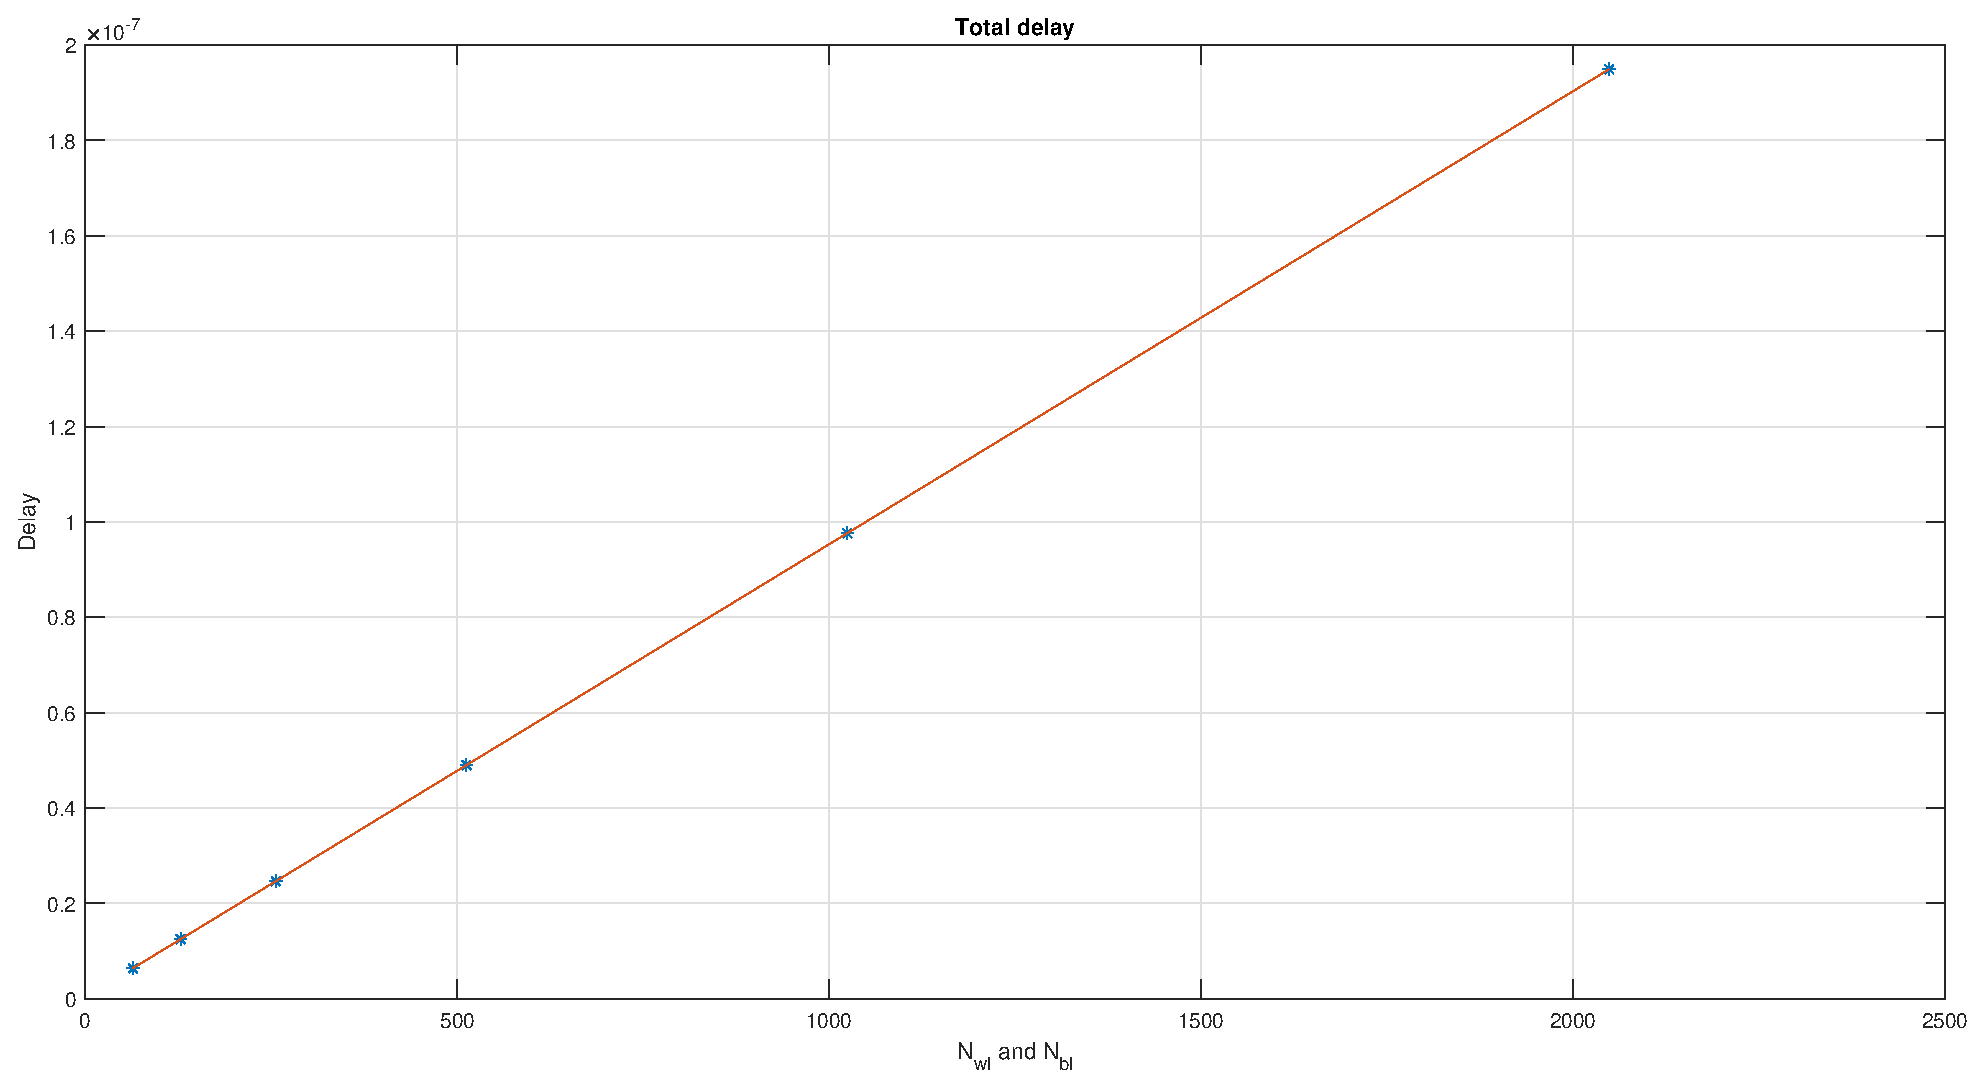
\includegraphics[scale=0.4]{delay_sim.eps}
	\end{center}
	\caption{Simulation of the delay varying the size of the memory array} 
\end{figure}

The behaviour represented is reasonable: in all the contributions previously discussed we always have at most a linear dependence on $N_{wl}$ or $N_{bl}$; some terms are independent from the variations of these two parameters and they partially contribute to the offset that can be observed on the 64x64 simulation point. Instead, we never have a square dependence on either of the two parameters, so an overall linear behaviour is perfectly reasonable.\\

So, with the values chosen for the parameters involved, the total delay of a precharge\&read operation spans between 6.43ns, in the 64x64 case, and 195ns in the 2048x2048 case.%Area
\chapter{Power Analysis}
\graphicspath{{foto/Chap3/}}

The estimation of power consumption is based on the analytical power
model described in [1].

\section{Capacitance modeling}
The considered capacitances are the following:
\begin{itemize}
	\item $C_{g,fg}$ gate capacitance of floating gate transistor
	\item $C_{d,fg}$ "drain/source" capacitance of floating gate transistor
	\item $C_{g,pt}$ gate capacitance of a generic pass transistor (SST and GST)
	\item $C_{d,pt}$ "drain/source" capacitance of a generic pass transistor (SST and GST)
	\item $C_{g,rowpass}$, $C_{g,colpass}$ and $C_{g,slice}$gate capacitance of SET and column pass transistors
	\item $C_{d,rowpass}$, $C_{d,colpass}$ and $C_{d,slice}$ drain capacitance of SET, column and slice pass transistors 
	\item $C_{wl,wire}$ wire capacitance per unit length of wordline
	\item $C_{bl,wire}$ wire capacitance per unit length of bitline
	\item $C_{ssl,wire}$ wire capacitance per unit length of string select line (the same for ground select line)
	\item $C_{slice,dec},C_{row,dec},C_{col,dec}$ total capacitances of each type of decoder
	\item $C_{SA,in}$ $C_{SA}$ input and load capacitance of the sense amplifier
	\item $C_{g,pre}$ gate capacitance of the precharge transtistor
	\item $C_{ext,pu\_driver}$ external precharge unit driver capacitance
\end{itemize}

Other useful parameters are:

\begin{itemize}
	\item $N_{bl}$ number of bitlines 
	\item $N_{wl}$ number of wordlines
	\item $L_{bl}$ length of bitline 
	\item $L_{wl}$ length of wordline
	\item $N_{slice}$ number of slices
	\item $N_{erase}$ number of erase cycles
\end{itemize}

\subsection{Floating gate transistor capacitances}

To evaluate power dissipation of a Floating Gate Transistor, the values of its capacitances are needed.\\
While in a traditional MOS structure there are Source, Drain and Gate capacitances, in a FGT there is a double gate structure (floating gate and control gate): the two capacitances $C_{fg}$ and $C_{cg}$ can be modeled as a single equivalent gate capacitance $C_{g,fg}$, series of the two and then equal to:

\[
C_{g,fg}=\frac{C_{fg} \cdot C_{cg}}{C_{fg}+C_{cg}}
\]

\subsection{Lines capacitances}
\label{subsec:capacitance}

To accurately evaluate the capacitance of the lines ($C_{bl}$ and $C_{wl}$), the capacitance of the wires  and the length of bitline/wordline are considered. So the total capacitance for each line is:

\[
C_{wl} = C_{d,rowpass} + C_{g,fg} \cdot N_{bl} + C_{wl,wire} \cdot L_{wl}
\]

\[
C_{bl}=2 \cdot C_{d,pt}+N_{wl}\cdot C_{d,fg}+C_{bl,wire} \cdot L_{bl} +C_{SA,in}
\]

where $C_{SA,in}$ is the input capacitance of the sense amplifier
\subsection{Decoders capacitance}
\label{subsec:dec_capacitance}
To evaluate the capacitance of the decoders, the following formulas are used:
\[
C_{slice,dec}=C_{d,sdec,pcharge}+C_{d,sdec,eval}+C_{g,sdec,inv_{p}}+C_{g,sdec,inv_{n}}
\]

\[
C_{slice,stack}=0.5 \cdot C_{g,sdec,n} \cdot Block\_Address \cdot N_{slice};
\]

where $C_{g,dec,eval}, C_{d,sdec,pcharge}$ and $C_{d,sdec,eval}$ are, respectively, the gate/drain capacitance of the precharge and evaluation transistors, while the others are the gate capacitances of the output inverter.
In particular, $C_{d,sdec,eval} = Block\_Address \cdot C_{d,sdec,n}$.\\
$C_{slice,stack}$ is the equivalent gate capacitance, that has to be loaded to turn on the n-mos and select the correct output, given certain selection bits from the address.\\
Similar expressions have been used for row and column decoders.
\subsection{Sense Amplifier}
\label{subsec:dec_capacitance}
To evaluate the capacitance of the sense amplifier, the following formulas are used:
\[
C_{SA,in}=C_{d,sa,p}+C_{d,sa,n}+C_{g,sa,p}+C_{g,sa,n}
\]

\[
C_{SA}=C_{d,colpass}+C_{d,slice}
\]

\section{Read Dynamic Power}
\label{sec:read_power}
\subsection{Decoding stage}
\label{sec:decoding_stage}
During a read operation, the slice decoder selects the slice in which the operation has to be carried out.
At the same time other two decoders, the row and the column one, are working to select the addressed word.
The formulas to calculate energy consumption in the decoding phase are the following:
\[
E_{slice,dec}= 0.5 \cdot C_{slice,dec} \cdot V_{on,pt}^2
\]
\[
E_{stack,sdec}=0.5 \cdot C_{slice,stack} \cdot V_{on,pt}^2
\]

\[
E_{row,dec}= 0.5 \cdot C_{row,dec} \cdot (V_{rd,sel}^2+ V_{rd,unsel}^2 \cdot (N_{wl}-1) + 2 \cdot V_{on,pt}^2) \cdot N_{slice}
\]
\[
E_{stack,rdec}=0.5 \cdot C_{row,stack} \cdot V_{on,pt}^2 \cdot N_{slice}
\]

\[
E_{col,dec}= 0.5 \cdot C_{col,dec} \cdot V_{on,pt}^2 \cdot N_{slice}
\]
\[
E_{stack,cdec}=0.5 \cdot C_{col,stack} \cdot V_{on,pt}^2 \cdot N_{slice}
\]

In this analysis, we are making the assumption that all the decoders have the same structure, but in reality the page decoder has a more complex one, having to give different voltages in output for each wordline.\\
The energy consumption linked to the selection of the slice and of the columns can be expressed as:
\[
E_{row,pt}= 0.5 \cdot (C_{g,rowpass} \cdot (N_{wl}+2) + N_{bit,word} \cdot C_{g,slice} ) \cdot V_{on,pt}^2
\]

\[
E_{col,pt}= 0.5 \cdot N_{bit,word} \cdot C_{g,colpass} \cdot V_{on,pt}^2
\]

\subsection{Precharge}
\label{sec:precharge}
In this state all the lines are isolated from the memory array and the bitlines are biased to a specific value $V_{bl,prec}$, by the precharge block, to speed up the following operation in order to reduce the latency. The other lines are biased to ground.\\
The formulas to calculate dissipated energy in the precharge phase are the following:

\[
E_{pre}= 0.5 \cdot (C_{ext,pu\_driver}+C_{g,pre}) \cdot V_{bl,prec}^2 \cdot N_bl
\]

\[
E_{bl}= 0.5 \cdot C_{bl,wire} \cdot L_{bl} \cdot V_{bl,prec}^2 \cdot N_{bl}
\]

\subsection{Read operation}
\label{sec:read_op}

The wordline of the selected page is biased to ground ($V_{rd,sel}$) while the voltage on the insulated page is set to $V_{rd,unsel}$. In this way the unselected pages act as a transfer gates and are always on independently from the values stored in the FGTs. It is assumed that the initial voltage of the wordline is 0.\\

The energy to switch the selected wordline is the following:
\[
E_{sel}= 0.5 \cdot C_{wl} \cdot V_{rd,sel} ^2
\]

The energy to switch the unselected wordlines is:
\[
E_{unsel}= 0.5 \cdot C_{wl}  \cdot V_{rd,unsel}^2 \cdot (N_{wl}-1)
\]

The bitlines are at the precharge voltage $V_{bl,prec}$ and are connected to the strings using SSTs and GSTs. Depending on the threshold voltage of the FGTs (1 or 0 stored) in the selected page, the bitlines can have two different kinds of voltage drop, $V_{rd,1}$ and $V_{rd,0}$. So a parameter that considers the distribution of 0s and 1s stored in the memory is used ($p_0$).\\

The energy to read a 1 is:
\[
E_1=0.5 \cdot C_{bl} \cdot (V_{bl,prec}-V_{rd,1})^2 \cdot N_{bl} \cdot (1-p_0)
\]

The energy to read a 0 is:
\[
E_0=0.5 \cdot C_{bl} \cdot (V_{bl,prec}-V_{rd,0})^2 \cdot N_{bl} \cdot p_0
\]

where $V_{bl,prec}-V_{rd,0}$, $V_{bl,prec}-V_{rd,1}$ are the voltage swing to the read of '0' and '1'.\\
The energy to activate SST and GST is:
\[
E_{pt}= 2 \cdot [0.5 \cdot C_{G,pt} \cdot V_{on,pt}^2] \cdot N_{bl}
\]
where $V_{on,pt}$ is the voltage to enable the pass transistors.

The energy on the string select line and ground select  line is:
\[
E_{sl}=E_{ssl}+ E_{gsl} = 2 \cdot [0.5 \cdot (C_{ssl,wire}\cdot L_{wl}) \cdot V_{on,pt}^2]
\]

\subsection{Sense Amplifier}
\label{sec:sense_amp}

The state change in the bitline is detected using a sense amplifier connected to each line.
The energy consumption related to this stage is given by:

\[
E_{SA}= 0.5 \cdot C_{SA} \cdot V_{bl,prec} \cdot ((V_{bl,prec}-V_{rd,0}) \cdot p_0 + (V_{bl,prec}-V_{rd,1}) \cdot (1-p_0)) \cdot N_bl
\]


\subsection{Total Power}
\label{sec:total_power}

Total energy is computed as summation of all the previous terms.
Assuming $f_{read}$ as read frequency and $E_{read}$as total read energy,, total read power can be computed as follows:
\[
P_{read}=E_{read}\cdot f_{read}
\]

\section{Write Dynamic Power}
\label{sec:write_power}
In the write stage, only the cells where the logical 0s will be written must be programmed, the others need to be inhibited. This can be performed by applying a voltage on the bitline that is 80\% of the voltage on the control gate ($V_{inhibit}$). The bitlines that need to be programmed with logical 0 are biased to ground. On all the control gates of the page a program voltage ($V_{prog}$) is applied. There is also a contribute due to tunneling energy $E_{tunnel}$.  It is assumed that the precharge voltage of the wordline is 0.\\

For the writing operation the column decoding is unneeded, being the page the smallest programmable unit. 
So the energy consumption for the decoding stage is given, as before, by the relations: 

\[
E_{slice,dec}= 0.5 \cdot C_{slice,dec} \cdot V_{on,pt}^2
\]
\[
E_{stack,sdec}=0.5 \cdot C_{slice,stack} \cdot V_{on,pt}^2
\]

\[
E_{row,pt}= 0.5 \cdot(C_{g,rowpass} \cdot (N_{wl}+2) + N_{bit,word} \cdot C_{g,slice} ) \cdot V_{on,pt}^2
\]

\[
E_{row,dec}= 0.5 \cdot C_{row,dec} \cdot (V_{prog}^2 + V_{inhibit}^2 \cdot (N_{wl}-1) + 2 \cdot V_{on,pt}^2) \cdot N_{slice}
\]
\[
E_{stack,rdec}=0.5 \cdot C_{row,stack} \cdot V_{on,pt}^2 \cdot N_{slice}
\]

The energy to precharge the bitlines is:
\[
E_{pre}= 0.5 \cdot C_{g,pre} \cdot V_{bl,prec}^2 \cdot N_{bl}
\]

\[
E_{bl}= 0.5 \cdot C_{bl,wire} \cdot L_{bl} \cdot V_{bl,prec}^2 \cdot N_{bl}
\]

The energy to switch the selected wordline is:

\[
E_{sel}=0.5 \cdot C_{wl} \cdot V_{prog}^2
\]

The energy to switch the unselected wordlines is:

\[
E_{unsel}=0.5 \cdot C_{wl} \cdot V_{inhibit}^2 \cdot (N_{wl}-1)
\]

The inhibit energy to maintain 1 in the cells is:

\[
E_{bl,inhibit}=0.5 \cdot (C_{bl}-C_{d,fg} \cdot N_{wl})\cdot (0.8 \cdot V_{inhibit})^2 \cdot N_{bl} \cdot (1-p_0)
\]

According to the self-boosted program inhibit model, the channel voltage is boosted to about $80\%$ of the applied control gate voltage by biasing the bit-lines corresponding to logical 1 at a specific voltage, in order to have that the boosted channel voltage is a fraction of the applied control gate voltage ($0.8 \cdot V_{inhibit}$).\\

The energy to program (write a 0) is:

\[
E_{bl,sel}= ( 0.5 \cdot (C_{bl}-C_{d,fg} \cdot N_{wl}) \cdot (0-V_{bl,prec})^2 + E_{tunnel}) \cdot N_{bl} \cdot p_0 
\]
The program voltage to be applied to the bitline is 0.\\


The energy to activate the pass transistors is:
\[
E_{pt}= 2 \cdot [0.5 \cdot C_{G,pt} \cdot V_{on,pt}^2] \cdot N_{bl}
\]
The energy on the string select line and ground select  line is:
\[
E_{sl}=E_{ssl}+ E_{gsl} = 2 \cdot [0.5 \cdot (C_{ssl,wire}\cdot L_{wl}) \cdot V_{on,pt}^2]
\]


In conclusion, the total amount of energy for a write operation is given by the addition of all these terms.\\
Assuming $f_{write}$ as write frequency and $E_{write}$as total write energy, total write power can be computed as follows:

\[
P_{write}=E_{write}\cdot f_{write}
\]


\section{Erase power}
\label{sec:erase_power}
For the erase operation, in planar flash NAND, the well of the block to erase is biased to an high voltage and the control gates are connected to ground. A high voltage is applied on the bitlines ($V_{prog}$) and the gates are biased to ground to have a tunnel effect that is in the opposite direction with respect to the write case. Also in this instance the tunnel energy must be considered.\\

Even in this case, the column decoding is unneeded and so the energy consumption is given, as before, by the relations: 

\[
E_{slice,dec}= 0.5 \cdot C_{slice,dec} \cdot V_{on,pt}^2
\]
\[
E_{stack,sdec}=0.5 \cdot C_{slice,stack} \cdot V_{on,pt}^2
\]

\[
E_{row,pt}= 0.5 \cdot (C_{g,rowpass} \cdot (N_{wl}+2) + N_{bit,word} \cdot C_{g,slice} ) \cdot V_{on,pt}^2
\]

\[
E_{row,dec}= 0.5 \cdot C_{row,dec} \cdot (V_{bl,erase}^2 \cdot N_{wl} + 2 \cdot V_{on,pt}^2) \cdot N_{slice}
\]
\[
E_{stack,rdec}=0.5 \cdot C_{row,stack} \cdot V_{on,pt}^2 \cdot N_{slice}
\]
The precharge step is required:
\[
E_{pre}= 0.5 \cdot C_{g,pre} \cdot V_{bl,prec}^2 \cdot N_bl
\]

\[
E_{bl}= 0.5 \cdot C_{bl,wire} \cdot L_{bl} \cdot V_{bl,prec}^2 \cdot N_{bl}
\]
The energy necessary to start erasing the block is:


\[
E_{erase,slice}=0.5 \cdot C_{bl} \cdot (V_{bl,erase}-V_{bl,prec})^2 \cdot N_{bl}+E_{tunnel} \cdot N_{bl} \cdot N_{wl}
\]
where $E_{tunnel} \cdot N_{bl} \cdot N_{wl}$ is the tunneling energy for the block.\\
The energy to activate the two pass transistors is the following:
\[
E_{pt}= 2 \cdot [0.5 \cdot C_{G,pt} \cdot V_{on,pt}^2] \cdot N_{bl}
\]

The energy on the string select line and ground select  line is:
\[
E_{sl}=E_{ssl}+ E_{gsl} = 2 \cdot [0.5 \cdot (C_{ssl,wire}\cdot L_{wl}) \cdot V_{on,pt}^2]
\]


Total energy for the erase operation is:

\[
E_{erase}=E_{slice,dec}+E_{stack,sdec}+E_{row,pt}+E_{stack,rdec}+E_{row,dec}+E_{bl}+(E_{erase,slice}+E_{pt}+E_{sl}) \cdot N_{erase}
\]	
where $N_{erase}$ is the number of erase cycles, necessary for the operation to be performed correctly.\\
Assuming $f_{erase}$ as erase frequency, total erase power can be computed as follows:
\[
P_{erase}=E_{erase}\cdot f_{erase}
\]

\section{Simulation results}
To verify the plausibility of our computations we assigned a reasonable value to each of the parameters involved in the equations.\\
In a first simulation the number of wordlines and bitlines change in a well defined range, to analyse how the power consumption changes if we vary the dimensions of the memory array. In particular, the array of values we considered for both $N_{wl}$ and $N_{bl}$, as for the delay, is $[64, 128, 256, 512, 1024, 2048]$. For each simulation point we assumed that $N_{bl}=N_{wl}$, because usually the memory arrays are made as square as possible, for reasons of space availability on the board.\\

The obtained results are reported in the following figures. 

\begin{figure}[H] 
	\begin{center}
		\includegraphics[scale=0.4]{Read_power_bl}
		\includegraphics[scale=0.4]{Write_power_bl}
	\end{center}
	\caption{Read Dynamic Power and Write Dynamic Power versus $N_{wl},N_{bl}$}
	\label{readwrite}
\end{figure}

\begin{figure}[H] 
	\begin{center}
		\includegraphics[scale=0.4]{Erase_power_bl}
	\end{center}
	\caption{Erase Dynamic Power versus $N_{wl},N_{bl}$}
\end{figure}

The behaviour represented is reasonable: in all the contributions previously discussed there is a more than linear dependence on $N_{wl}$ and $N_{bl}$. In particular the most relevant contributions are dependent from the product of these two parameters, giving as result a quadratic curve.\\
The curves in Figure \ref{readwrite} show that power consumption for read and write operations is in the order of some $\mu W$, while the erase power is about one order of magnitude larger.\\
In a second analysis $N_{wl}$ and $N_{bl}$ are fixed, with a value of 1024, while $N_{slice}$ varies according to the values $[32, 64, 128, 256]$.
\begin{figure}[H] 
	\begin{center}
		\includegraphics[scale=0.4]{Read_power_slice}
		\includegraphics[scale=0.4]{Write_power_slice}
	\end{center}
	\caption{Read Dynamic Power and Write Dynamic Power versus $N_{slice}$}
\end{figure}

\begin{figure}[H] 
	\begin{center}
		\includegraphics[scale=0.4]{Erase_power_slice}
	\end{center}
	\caption{Erase Dynamic Power versus $N_{slice}$}
\end{figure}

As it can be seen, the dependency from $N_{slice}$ is linear. However, having supposed that all the unselected blocks are deactivated, the increase in the curves is due to the power consumption of an higher number of decoders.%Delay
\chapter{Area and Volume}
\graphicspath{{foto/Chap4/}}
In this chapter we have computed the area and the volume of the complete structure of the register file (10T Cell, Decoders and Sense Amplifier).

\section{Memory Block}
For the area and volume evaluation of the memory, the model in figure \ref{fig:cube} has been used.

\begin{center}
	\begin{figure}[H]
		\centering
		\includegraphics[scale = 0.9, trim={0 5cm 10cm 0},clip]{cube}
		\caption{Simplified Register File structure}
		\label{fig:cube}
	\end{figure}
\end{center}

The three dimensions of the array have been computed as follows:

\begin{itemize}
	\item \textit{Width, Length}: In order to find these values, the area of the elementary bit cell has been calculated and then its square root has been used in order to compute width and length.
	\[
	\textbf{Area\_BitCell}=2 \cdot (N\_port\_Wr+N\_port\_Rd) \cdot Tr\_n\_Area +
	\]
	\[
	+ 2 \cdot (Tr\_n\_Area + Tr\_p\_Area)
	\]
	\[
	\textbf{W}=(2 \cdot (N\_port\_Wr + N\_port\_Rd) \cdot Pitch_{pp} + \sqrt{Area\_BitCell}) \cdot N_{bit} +
	\]
	\[
	+ Pitch_{pp} \cdot (N_{bit}-1)
	\]
	\[
	\textbf{L}=N_{block} \cdot Pitch_{pp}
	\]
	
	As it can be seen, the area of the SRAM memory cell is computed as function of the number of read and write ports. Other elements, influenced by the number of input ports, are the number of wordline and bitline: this will affect the width and, as it can be seen in the following step, the height of the memory block.
	
	\item \textit{Height of the stack}: the terms considered are the height of the Cells that takes into account of the the number of Read and Write lines and their distances, the square root of the Area of bit cells, and the distance between them, as shown in \ref{fig:Stack}.
	\[
	\textbf{H}=((N\_port\_Wr+N\_port\_Rd) \cdot Pitch_{pp} + \sqrt{Area\_BitCell}) \cdot N_{bit} +
	\]
	\[
	+ Pitch_{pp} \cdot (N_{bit}-1)	
	\]
	
Finally, the area and the volume of the Register File can be calculated as:
	\[
	\textbf{Memory\_Array\_Area}=H \cdot W
	\]
	\[
	\textbf{Memory\_Array\_Volume}=H \cdot W \cdot L
	\]
	
\begin{center}
	\begin{figure}[H]
		\centering
		\includegraphics[scale = 0.4]{section_pillars}
		\caption{Stack structure}
		\label{fig:Stack}
	\end{figure}
\end{center}
\end{itemize}

\section{Decoders}
For the area and volume evaluation of all the decoders, the model that has been used is the same described in the Chapter 2. For each decoder the number of n-type transistors was first calculated and then the number of p-type transistors; subsequently they have been multiplied by their minimum area value and then added together to calculate the total area. Finally the volume has been calculated as the multiplication of the Area and the length.

\begin{itemize}
\item{\textbf{Block Decoder}}:
The area of the \textit{Block Decoder} has been calculated as: area of the the core of the decoder added to the area of the inverter connected at the input and and at the output. In this case the number of input is given by the \textit{Block Address} while the output is equal to the number of slice $N_{slice}$. The volume is the area multiplied by the single distance between two transistor because there is only one \textit{Block Decoder}. So:
	\[
	\#Tr\_n\_Block\_Dec = Block\_Address \cdot N_{slice} + N_{slice} + Block\_Address
	\]
	\[
	\#Tr\_p\_Block\_Dec = 2 \cdot N_{slice} + Block\_Address
	\]
	\\
	\[
	\textbf{Block\_Dec\_Area} = \#Tr\_n\_Block\_Dec \cdot Tr\_n\_Area +
	\]
	\[
	+ \#Tr\_p\_Block\_Dec \cdot Tr\_p\_Area
	\]
	\[
	\textbf{Block\_Dec\_Volume} = Block\_Dec\_Area \cdot Pitch_{pp}
	\]

\item{\textbf{Row Decoder}}:
The area of the \textit{Row Decoder} has been calculated as before but in this case the number of input is done by the \textit{Row Address} while the output is equal to the number of row that is $(N_{wl})$. This is finally multiplied by the total number of read and write ports. The volume is the area multiplied by the length. So:
	\[
	\#Tr\_n\_Row\_Dec = Row\_Address \cdot N_{wl} + N_{wl} + Row\_Address
	\]
	\[
	\#Tr\_p\_Row\_Dec = 2 \cdot N_{wl} + Row\_Address
	\]
	\\
	\[
	\textbf{Row\_Dec\_Area} = (N\_port\_Wr+N\_port\_Rd) \cdot (\#Tr\_n\_Row\_Dec \cdot Tr\_n\_Area +
	\]
	\[
	+ \#Tr\_p\_Row\_Dec \cdot Tr\_p\_Area)
	\]
	\[
	\textbf{Row\_Dec\_Volume} = Row\_Dec\_Area \cdot L
	\]
\newpage

\item{\textbf{Decoder Address}}:
The previous variables $Block\_Address$, $Row\_Address$,\\ $N\_wl$ and $N\_block$ are computed as:

	\[
	Block\_Address = ceil(log_{2}(N_{block}))
	\]
	\[
	Row\_Address = ceil(log_{2}(N_{wl}))
	\]
	\[
	N\_wl=min(N\_word,N\_bit)
	\]
	\[
	N\_block = ceil \Bigl ( \frac{N\_word} {N\_bit}\Bigl )
	\]

\end{itemize}
\section{Bit Line Inverters, Pass Transistors \\and Precharge Transistors}
In the total structure there are some pass transistor of n-type used to help the selection of the wanted memory cell.
\begin{itemize}
\item{\textbf{Bit Line Inverters}}:
The area has been calculated as $N_{bl}$ multiplied by the area of single p-type and n-type transistor p-type and n-type and then multiplied by the total number of read and write ports, while the volume is the area multiplied by the length. So:
	\[
	\textbf{Inverter\_bl\_Area} = (N\_port\_Wr+N\_port\_Rd) \cdot \cdot (N_{bl} \cdot Tr\_n\_Area +
	\]
	\[
	+ N_{bl} \cdot Tr\_p\_Area)
	\]
	\[
	\textbf{Inverter\_bl\_Volume} = Inverter\_bl\_Area \cdot L
	\]

\item{\textbf{Row Pass Transistors}}:
The area has been calculated as $N_{wl}$ multiplied by the area of single transistor and then multiplied by the total number of read and write ports, while the volume is the area multiplied by the length. So:
	\[
	\textbf{Pass\_Row\_Area} = (N\_port\_Wr+N\_port\_Rd) \cdot N_{wl} \cdot Tr\_n\_Area
	\]
	\[
	\textbf{Pass\_Row\_Volume} = Pass\_Row\_Area \cdot L
	\]
\item{\textbf{Column Pass Transistors}}:
The area has been calculated as $N_{bl}$ multiplied by the area of single transistor and then multiplied by the total number of read ports, while the volume is the area multiplied by the length. So: 
	\[
	\textbf{Pass\_Column\_Area} = N\_port\_Rd \cdot N_{bl} \cdot Tr\_n\_Area
	\]
	\[
	\textbf{Pass\_Column\_Volume} = Pass\_Column\_Area \cdot L
	\]
\item{\textbf{Slice Pass Transistors}}:
The area is the area of single transistor and then multiplied by the total number of read ports, while the volume is the area multiplied by the length. So:
	\[
	\textbf{Pass\_Slice\_Area} = N\_port\_Rd \cdot Tr\_n\_Area
	\]
	\[
	\textbf{Pass\_Slice\_Volume} = Pass\_Slice\_Area \cdot L
	\]
\item{\textbf{Precharge Transistors}}:
The area has been calculated as $N_{bl}$ multiplied by the area of single p-type transistor and then multiplied by the total number of read ports, while the volume is the area multiplied by the length. So:
	\[
	\textbf{Precharge\_Area} = N\_port\_Rd \cdot N_{bl} \cdot Tr\_p\_Area
	\]
	\[
	\textbf{Precharge\_Volume} = Precharge\_Area \cdot L
	\]
\end{itemize}

\section{Sense Amplifier}
The area of the two \textit{Sense Amplifiers} has been calculated as remembering the structure described in Chapter 2 and the volume is the area multiplied by the length. So:

	\[
	\#Tr\_n\_SA=N_{bl} \cdot 3
	\]
	\[
	\#Tr\_p\_SA=N_{bl} \cdot 3
	\]
	\\
	\[
	\textbf{SA\_Area} = N\_port\_Rd \cdot (\#Tr\_n\_SA \cdot Tr\_n\_Area + \#Tr\_p\_SA \cdot Tr\_p\_Area)
	\]
	\[
	\textbf{SA\_Volume} = SA\_Area \cdot L
	\]

\section{Total Area and Total Volume}
The total area has been calculated has the sum of the area of the memory array and all the boundary circuits:
	\[
	\textbf{Total\_Area}= Memory\_Array\_Area + Block\_Dec\_Area + Row\_Dec\_Area + 
	\]
	\[
	+ Pass\_Row\_Area + Pass\_Column\_Area + Pass\_Slice\_Area +
	\]
	\[
	+ Inverter\_bl\_Area +  SA\_Area
	\]
The total volume has been calculated has the sum of the volume of the memory array and all the boundary circuits:
	\[
	\textbf{Total\_Volume}= Memory\_Array\_Volume + Block\_Dec\_Volume + Row\_Dec\_Volume + 
	\]
	\[
	+ Pass\_Row\_Volume + Pass\_Column\_Volume + Pass\_Slice\_Volume +
	\]
	\[
	+ Inverter\_bl\_Volume +  SA\_Volume
	\]
\section{Simulation result}
In order to verify the the computations made before, it has been made a simulation; in particular it has been reported two graphs in which are represented how the area and the volume change with the only value of $N_{bit}$ since the assumption is that the Register File is a perfect cube. In particular, the array of values it has been considered for $N_{bit}$ is $[8, 16, 32, 64, 128]$.
\\The behaviours represented are reasonable: in the two graphs \ref{fig:1} and \ref{fig:2} there is a square dependency. Changing the value of this parameter, the total area increases quadratically and the volume increase quadratically too.\\
The obtained results are reported in the following figures.

\begin{center}
	\begin{figure}[H]
		\centering
		\includegraphics[scale=0.4]{Total_Area.png}
		\caption{Simulation of the Total Area value, varying the number of bit.} 
		\label{fig:1}
	\end{figure}
\end{center}

\begin{center}
	\begin{figure}[H]
		\centering
		\includegraphics[scale=0.4]{Total_Volume.png}
		\caption{Simulation of the Total Volume value, varying the number of bit.}
		\label{fig:2} 
	\end{figure}
\end{center}

%Power
\chapter{Matlab code}

\section{InputParameters.m}
\inputminted[linenos=true, 
bgcolor=bgcode,
frame=lines,
framesep=2mm,
baselinestretch=1.2,
fontsize=\footnotesize,
breaklines,
]{matlab}{Code/InputParameters.m}

\section{Memories3D.m}
\inputminted[linenos=true, 
bgcolor=bgcode,
frame=lines,
framesep=2mm,
baselinestretch=1.2,
fontsize=\footnotesize,
breaklines,
]{matlab}{Code/Memories3D.m}%Power


\end{document}